\chapter{Evaluation} 
This chapter goes over the methodology used to evaluate the different patterns, and also talks about what data has been collected, which would be the basis for the following chapter. 

\section{Cloud Configuration}
% https://docs.microsoft.com/en-us/azure/virtual-machines/av2-series 
% https://docs.microsoft.com/en-us/azure/virtual-machines/sizes-b-series-burstable
% https://docs.microsoft.com/en-us/azure/virtual-machines/sizes-general
The applications are evaluated on the Azure cloud platform under two different patterns. To ensure a fair test the applications were deployed on five different machine types where possible, each machine different amount of vCPUs and memory size (RAM), however with a standardised amount of storage set at 60GB and all machines were hosted in the UK South region. 

Three of the five machines are use machines from the Av2-series set, where it's size is throttled based on the hardware to provide consistent processor performance for the running instance, which are best suited for the likes of a low traffic web server, proofs-of-concept application, and code repositories.

The other two machines use machines from the B-series burstable machines set, which are ideal for workloads that do not require full CPU continuity performance, the burstable feature allows for the baseline CPU performance to burst at a higher level to support spiked up loads,  such machines are useful with web servers or small databases. 

The load machines were all created on the Standard\_A2\_v2 machines, within the same regions allowing to use load generators for the applications without having an interrupted connection to the servers, using load machines on the cloud allowed to run multiple machines at the same time decreasing the amount of time it took to collect data. 

The below table provides a list of configurations used through the testing process.  

\begin{table}[H]
    \centering % used for centering table
    \begin{tabular}{c c c c} % centered columns (4 columns)
    \toprule\toprule %inserts double horizontal lines
     Machine Name & vCPUs & Memory & Cost_{/hr} \\ [0.5ex] % inserts table
    %heading
    \hline % inserts single horizontal line
    Standard\_A2\_v2 & 2  & 4  & \pounds 0.08 \\ [0.5ex] 
    Standard\_A4\_v2 & 4  & 8  & \pounds 0.17 \\ [0.5ex] 
    Standard\_A8\_v2 & 8  & 16 & \pounds 0.34 \\ [0.5ex] 
    Standard\_B12ms & 12 & 48 & \pounds 0.42 \\  [0.5ex] 
    Standard\_B16ms & 16 & 64 & \pounds 0.56 \\  [0.5ex] 
    \toprule %inserts single line
    \end{tabular}
    \label{table:nonlin} % is used to refer this table in the text
    \caption{Azure Machine Specifications} % title of Table

\end{table}


\section{Naming Convention}
To simplify different combinations of patterns and applications, a mixture of fruits that make up a fruit cocktail juice has been used to name each combination, these have been identified in the following table:

\begin{table}[H]
    \caption{Naming Convention} % title of Table
    \centering % used for centering table
    \begin{tabular}{>{\raggedright\arraybackslash}c c c} % centered columns (3 columns)
        \hline %inserts double horizontal lines
        Name & Application & Pattern  \\ [0.5ex] % inserts table 
        %heading
        \hline% inserts single horizontal line
        Pineapple   & Robot Shop     & Pattern One \\  [0.5ex] 
        Lime        & Robot Shop     & Pattern Two \\  [0.5ex] 
        Orange      & Social Network & Pattern One \\  [0.5ex] 
        Mango       & Social Network & Pattern Two \\  [0.5ex] 
        Watermelon  & Hotel Reservation  & Pattern One \\  [0.5ex] 
        Grape       & Hotel Reservation  & Pattern Two \\  [0.5ex] 
    
        \hline %inserts single line
    \end{tabular}
    \label{table:nonlin} % is used to refer this table in the text
\end{table}

\section{Collected Data}

\begin{table}[ht!]
 % title of Table
    \centering % used for centering table
    \begin{tabular}{c c c c c c c} % centered columns (4 columns)
    \hline %inserts double horizontal lines
             & Pineapple & Orange & Watermelon & Lime  & Grape & Mango \\ [0.5ex] % inserts table
    %heading
    \hline% inserts single horizontal line
    Standard\_A2\_v2 & Yes & Yes & Yes & Yes & Yes & Yes  \\  [0.5ex] 
    Standard\_A4\_v2 & Yes & Yes & Yes & Yes & Yes & Yes  \\  [0.5ex] 
    Standard\_A8\_v2 & Yes & Yes & Yes & Yes & Yes & Yes  \\  [0.5ex] 
    Standard\_B12ms  & Yes & Yes & Yes  & No & No  & No  \\  [0.5ex] 
    Standard\_B16ms  & Yes & Yes & Yes  & No & No  & No  \\  [0.5ex] 
    \hline %inserts single line
    \end{tabular}
    \caption{
This table identifies collected data from each combination, a few of the machines were unable to collect certain data due to the B-Tier machines having a strict quota limit which made it impossible to run enough machines to have an adequate amount of runs to collect of data.}
    \label{table:nonlin} % is used to refer this table in the text
\end{table}






\section{Results}
\subsection{Robot Shop Results}
\begin{figure}[H]
     \centering
     \begin{subfigure}[b]{0.49\textwidth}
         \centering
         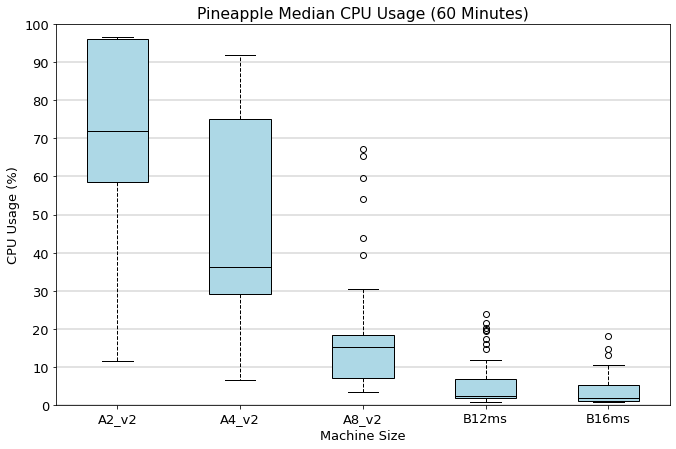
\includegraphics[width=\textwidth]{images/pineapple_cpu.png}
         \caption{Pineapple}
         \label{fig:pineapple_cpu}
     \end{subfigure}
     \hfill
     \begin{subfigure}[b]{0.49\textwidth}
         \centering
         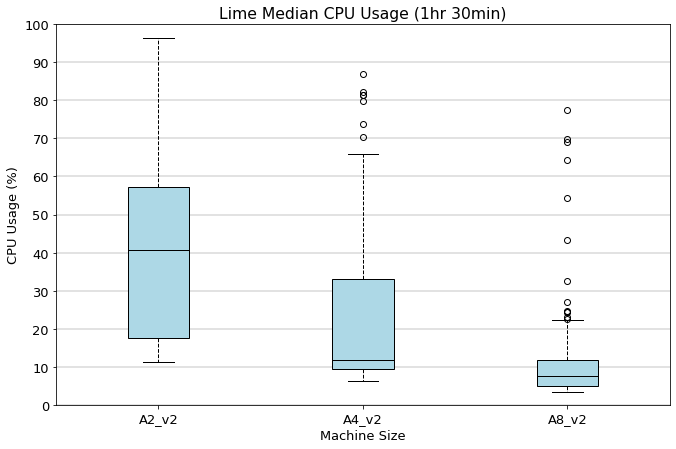
\includegraphics[width=\textwidth]{images/lime_cpu.png}
         \caption{Lime}
         \label{fig:lime_cpu}
     \end{subfigure}
    
        \caption{Part 1 Server CPU Usage(Average)}
        \label{fig:part_1_cpu}
\end{figure}
\begin{figure}[H]
     \centering
     \begin{subfigure}[b]{0.49\textwidth}
         \centering
         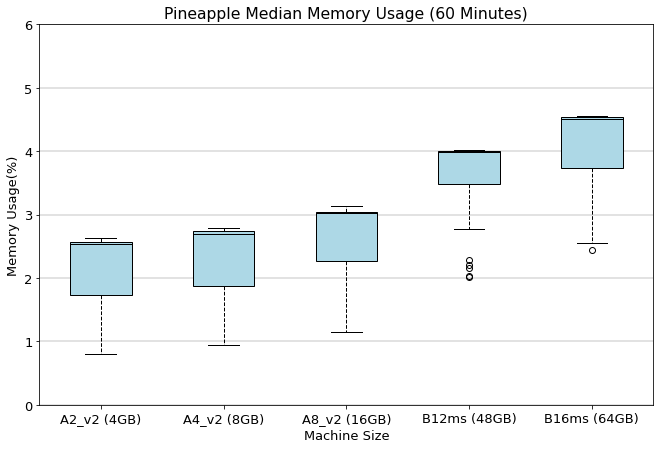
\includegraphics[width=\textwidth]{images/pineapple_mem.png}
         \caption{Pineapple}
         \label{fig:pineapple_cpu}
     \end{subfigure}
     \hfill
     \begin{subfigure}[b]{0.49\textwidth}
         \centering
         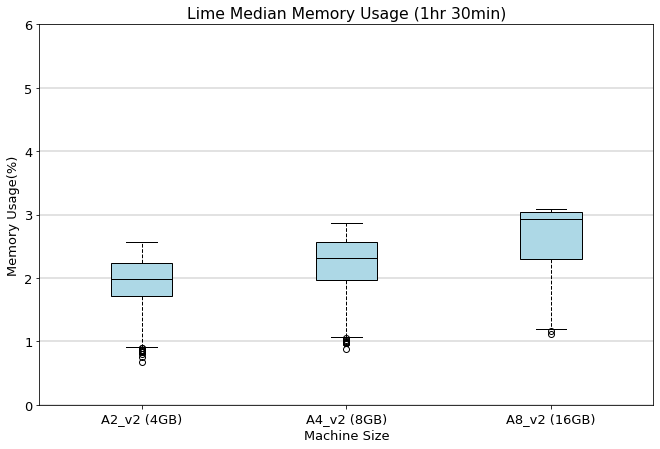
\includegraphics[width=\textwidth]{images/lime_mem.png}
         \caption{Lime}
         \label{fig:lime_cpu}
     \end{subfigure}
    
        \caption{Part 1 Server Memory Usage(Average)}
        \label{fig:part_1_cpu}
\end{figure}
\begin{figure}[H]
     \centering
     \begin{subfigure}[b]{0.49\textwidth}
         \centering
         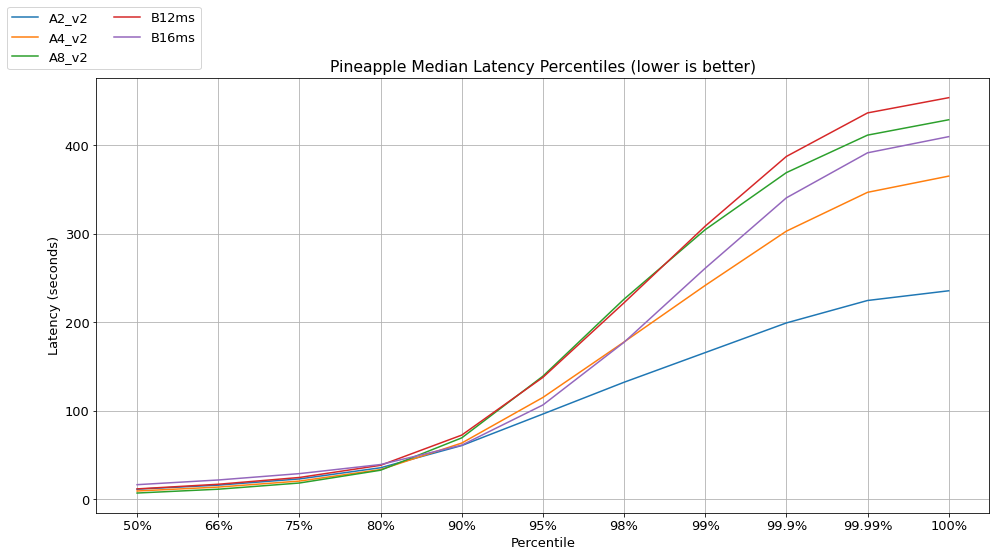
\includegraphics[width=\textwidth]{images/pineapple_latency.png}
         \caption{Pineapple} 
         \label{fig:pineapple_cpu}
     \end{subfigure}
     \hfill
     \begin{subfigure}[b]{0.49\textwidth}
         \centering
         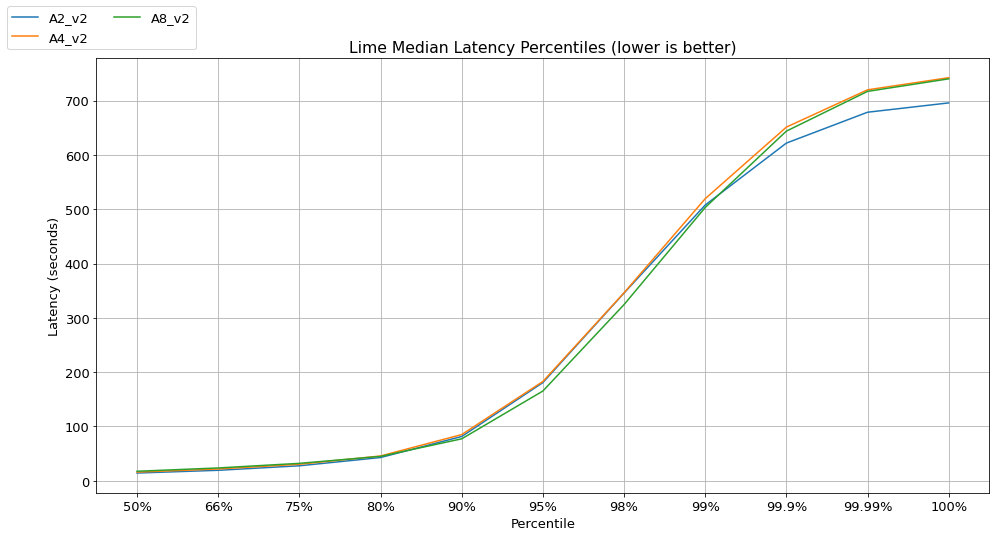
\includegraphics[width=\textwidth]{images/lime_latency.png}
         \caption{Lime}
         \label{fig:lime_cpu}
     \end{subfigure}
    
        \caption{Part 1 Load Generator Latency Graphs(Average)}
        \label{fig:part_1_cpu}
\end{figure}
% =======================
% =======================
\subsection{Social Network Results}
\begin{figure}[H]
     \centering
     \begin{subfigure}[b]{0.49\textwidth}
         \centering
         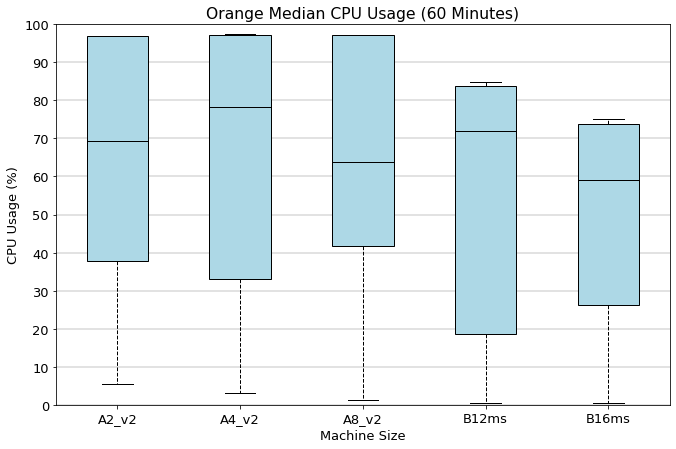
\includegraphics[width=\textwidth]{images/orange_cpu.png}
         \caption{orange}
         \label{fig:orange_cpu}
     \end{subfigure}
     \hfill
     \begin{subfigure}[b]{0.49\textwidth}
         \centering
         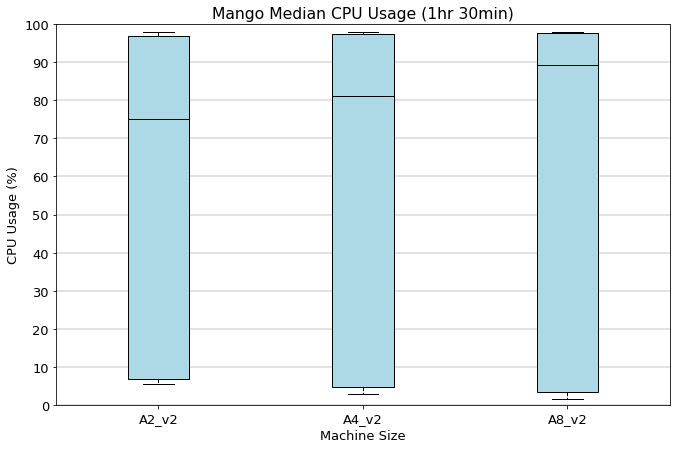
\includegraphics[width=\textwidth]{images/mango_cpu.png}
         \caption{mango}
         \label{fig:mango_cpu}
     \end{subfigure}
    
        \caption{Part 2 Server CPU Usage(Average)}
        \label{fig:part_2_cpu}
\end{figure}
\begin{figure}[H]
     \centering
     \begin{subfigure}[b]{0.49\textwidth}
         \centering
         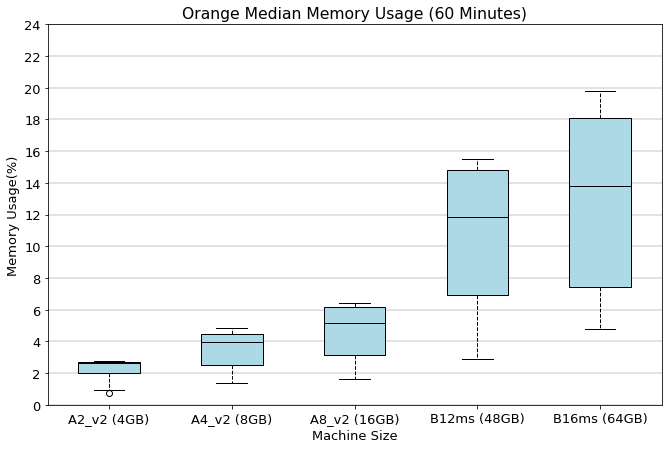
\includegraphics[width=\textwidth]{images/orange_mem.png}
         \caption{orange}
         \label{fig:orange_mem}
     \end{subfigure}
     \hfill
     \begin{subfigure}[b]{0.49\textwidth}
         \centering
         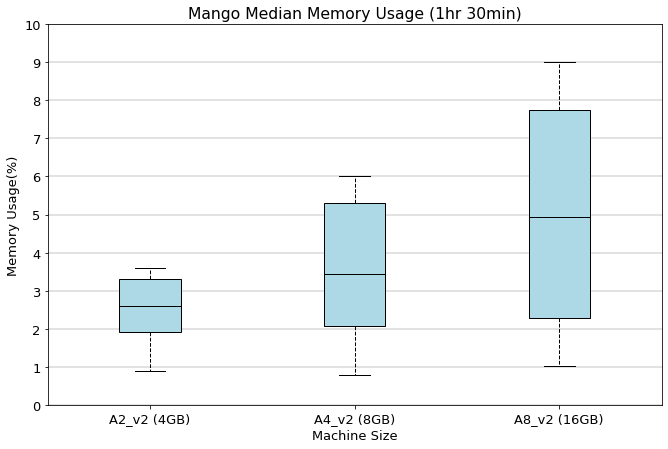
\includegraphics[width=\textwidth]{images/mango_mem.png}
         \caption{mango}
         \label{fig:mange_mem}
     \end{subfigure}
    
        \caption{Part 2 Server Memory Usage(Average)}
        \label{fig:part_2_mem}
\end{figure}
\begin{figure}[H]
     \centering
     \begin{subfigure}[b]{0.49\textwidth}
         \centering
         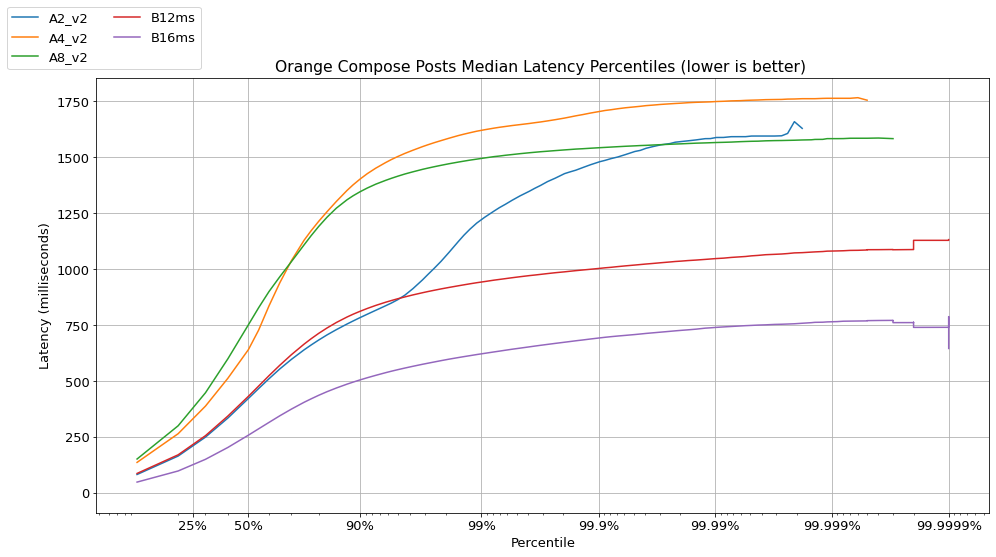
\includegraphics[width=\textwidth]{images/orange_compose.png}
         \caption{orange} 
         \label{fig:orange_compose}
     \end{subfigure}
     \hfill
     \begin{subfigure}[b]{0.49\textwidth}
         \centering
         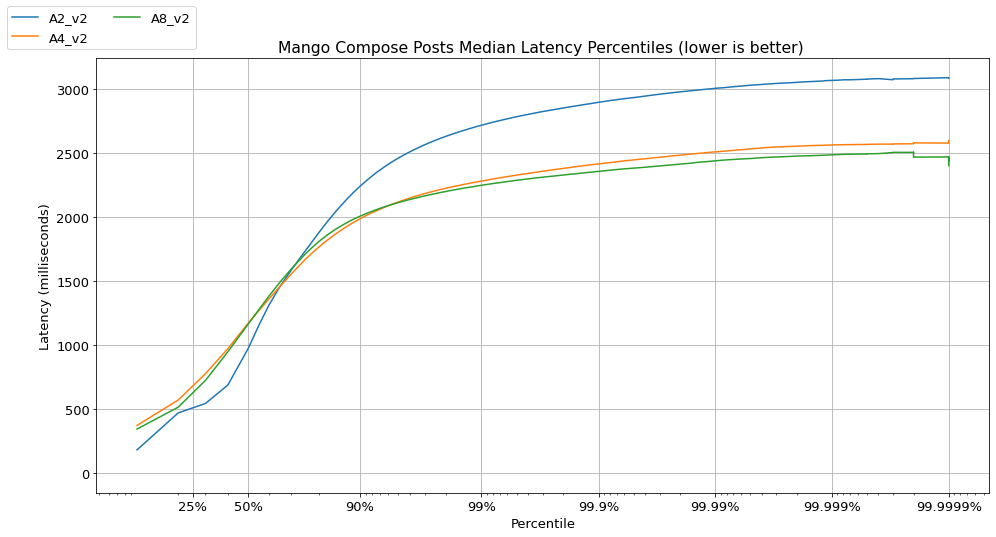
\includegraphics[width=\textwidth]{images/mango_compose.png}
         \caption{mango}
         \label{fig:mango_compose}
     \end{subfigure}
    
        \caption{Part 2 Load Generator (Compose) Latency Graphs(Average)}
        \label{fig:part_2_compose}
\end{figure}
\begin{figure}[H]
     \centering
     \begin{subfigure}[b]{0.49\textwidth}
         \centering
         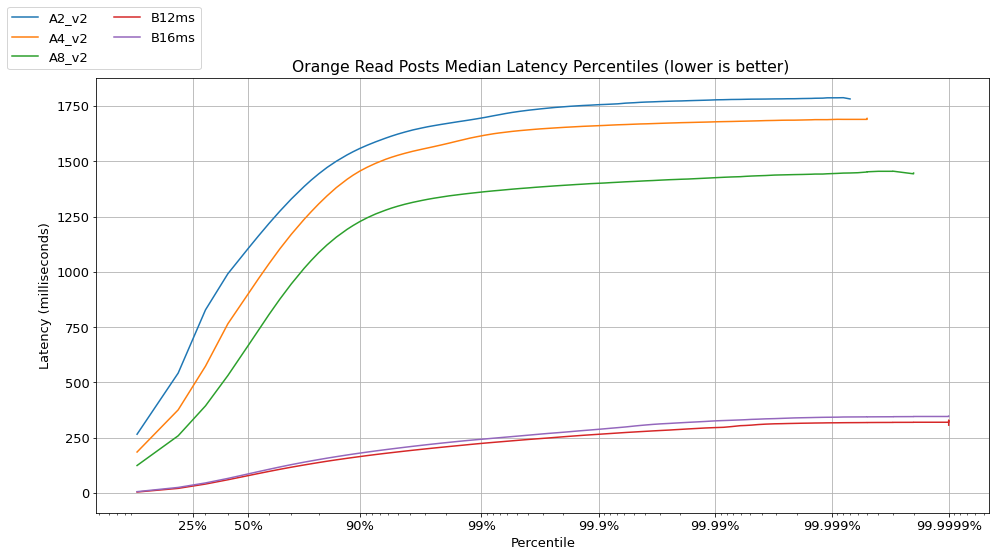
\includegraphics[width=\textwidth]{images/orange_read.png}
         \caption{Orange} 
         \label{fig:orange_read}
     \end{subfigure}
     \hfill
     \begin{subfigure}[b]{0.49\textwidth}
         \centering
         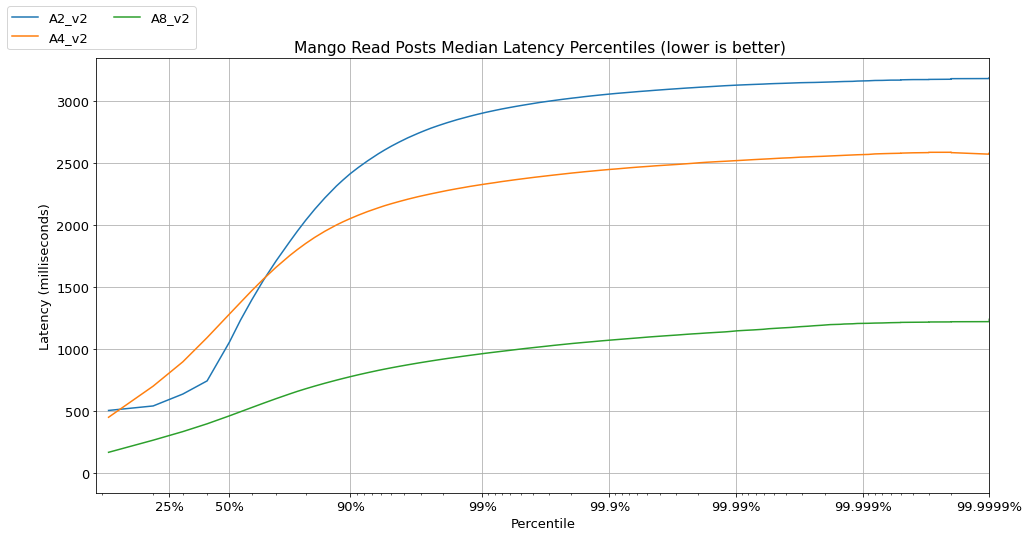
\includegraphics[width=\textwidth]{images/mango_read.png}
         \caption{Mango}
         \label{fig:mango_read}
     \end{subfigure}
    
        \caption{Part 1 Load Generator (Read) Latency Graphs  (Average)}
        \label{fig:part_2_read}
\end{figure}

\section{Hotel Reservation Results }
\begin{figure}[H]
     \centering
     \begin{subfigure}[b]{0.49\textwidth}
         \centering
         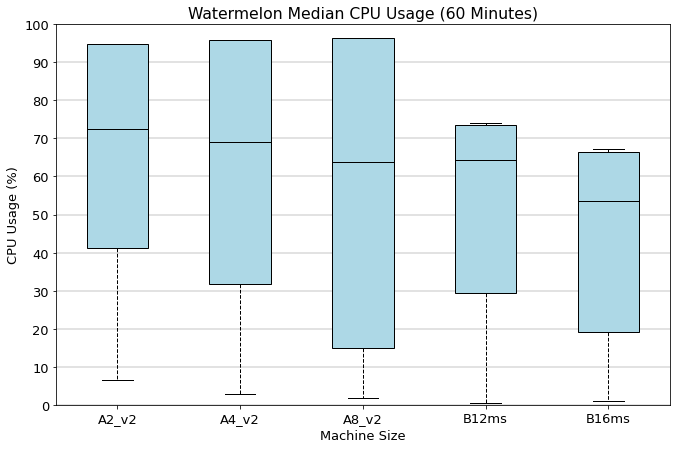
\includegraphics[width=\textwidth]{images/watermelon_cpu.png}
         \caption{watermelon}
         \label{fig:watermelon_cpu}
     \end{subfigure}
     \hfill
     \begin{subfigure}[b]{0.49\textwidth}
         \centering
         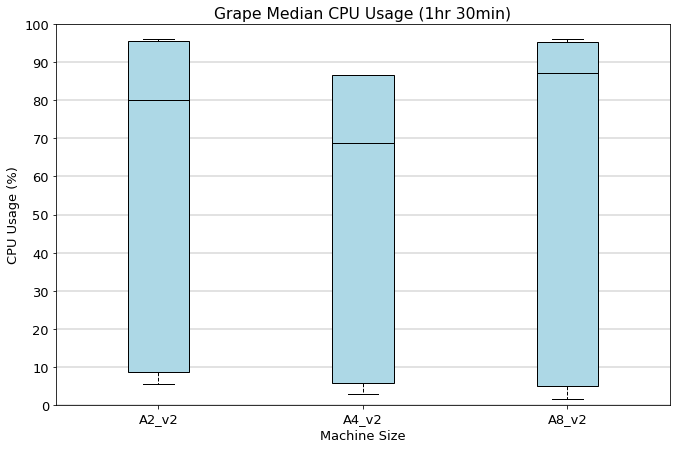
\includegraphics[width=\textwidth]{images/grape_cpu.png}
         \caption{grape}
         \label{fig:grape_cpu}
     \end{subfigure}
    
        \caption{Part 3 Server CPU Usage (Average)}
        \label{fig:part_3_cpu}
\end{figure}
\begin{figure}[H]
     \centering
     \begin{subfigure}[b]{0.49\textwidth}
         \centering
         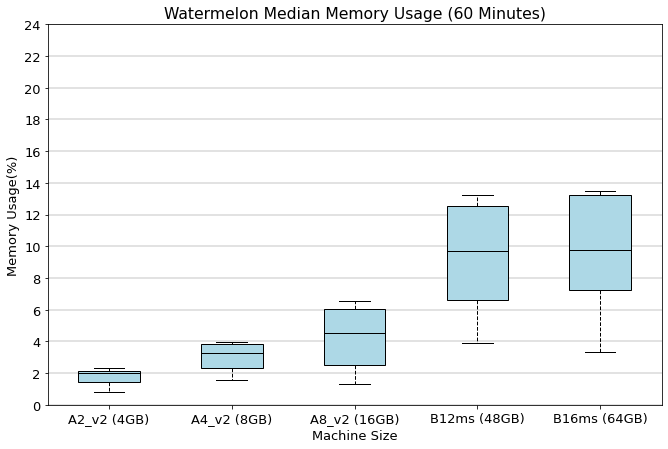
\includegraphics[width=\textwidth]{images/watermelon_mem.png}
         \caption{orange}
         \label{fig:watermelon_mem}
     \end{subfigure}
     \hfill
     \begin{subfigure}[b]{0.49\textwidth}
         \centering
         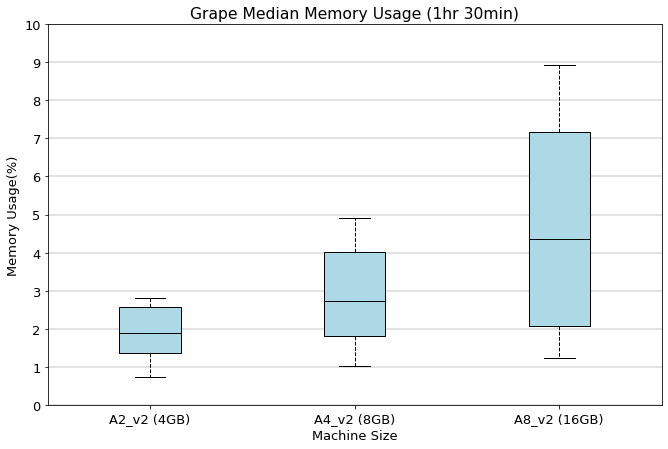
\includegraphics[width=\textwidth]{images/grape_mem.png}
         \caption{grape}
         \label{fig:grape_mem}
     \end{subfigure}
    
        \caption{Part 3 Server Memory Usage (Average)}
        \label{fig:part_3_mem}
\end{figure}
\begin{figure}[H]
     \centering
     \begin{subfigure}[b]{0.49\textwidth}
         \centering
         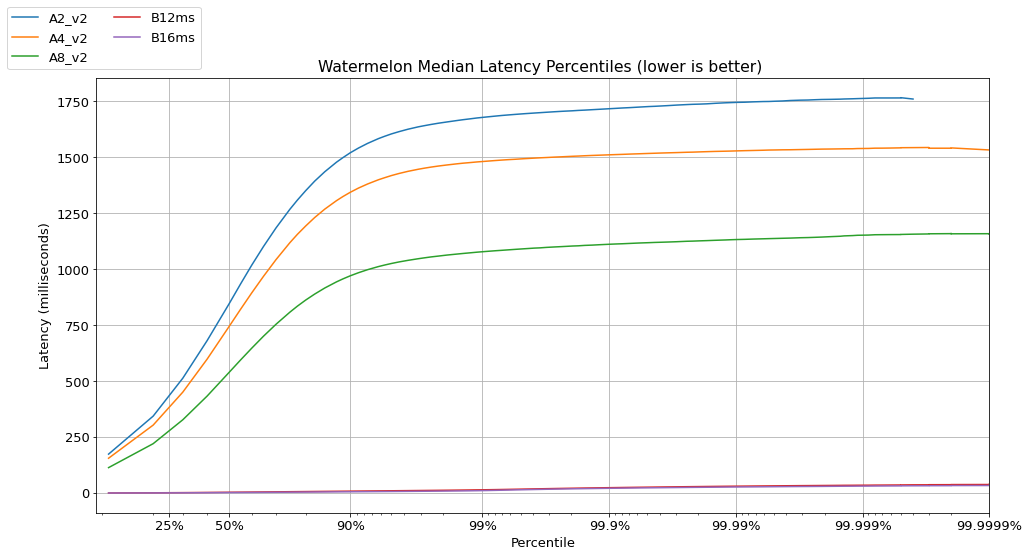
\includegraphics[width=\textwidth]{images/watermelon_latency.png}
         \caption{Pineapple} 
         \label{fig:watermelon_compose}
     \end{subfigure}
     \hfill
     \begin{subfigure}[b]{0.49\textwidth}
         \centering
         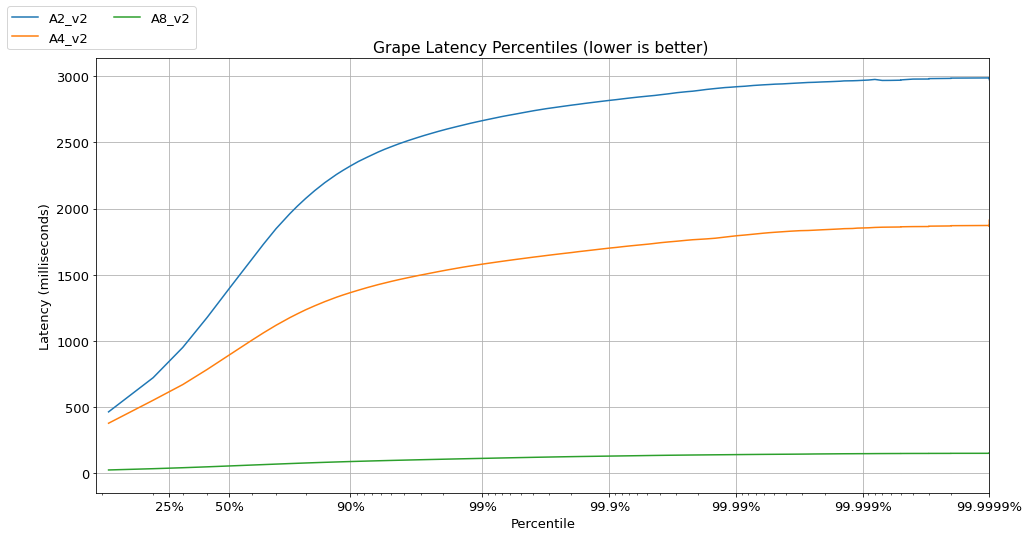
\includegraphics[width=\textwidth]{images/grape_latency.png}
         \caption{Lime}
         \label{fig:grape_compose}
     \end{subfigure}
    
        \caption{Part 3 Load Generator Latency Graphs (Average)}
        \label{fig:part_3_compose}
\end{figure}

\section{Do different patterns throttle applications more?}
\section{Do different patterns scale well with increased machine hardware}
\section{Depending on the number of services, would if be cost effective to use different machines}

\chapter{Analysis}